\documentclass{article}

\usepackage{tikz}
\usepackage{standalone}
\usepackage{pgfplots}
\pgfplotsset{compat=newest}
\usepackage{tikz}
\usetikzlibrary{decorations.markings}

\usepackage{subcaption}
\usepackage[margin=2.5cm]{geometry}
\usepackage{amsmath}
\usepackage{amssymb}


\newcommand\greybox[1]{
	\vskip\baselineskip
	\par\noindent\colorbox{lightgray}{
		\begin{minipage}{\textwidth}#1\end{minipage}
	}
	\vskip\baselineskip
}

\title{Forelesning 2}


\begin{document}
\maketitle

\section{Schrödinger ligningen}

Vi starter med å skrive opp Schrödingers berømte bevegelsesligning for en enkelt partikkel
i et potensial $V(x)$ som
\begin{align}
	 -\frac{\hbar^2}{2m}\frac{\partial^2 \Psi(x,t)}{\partial x^2} + V(x)\Psi(x,t) =
	i\hbar \frac{\partial \Psi(x,t)}{\partial t} 
\end{align}
hvor $m$ er partikkelens masse og $\hbar=\frac{h}{2\pi}$.
$\Psi(x,t)$ er partikkelens bølgefunksjon, som vi skal se bestemmer hvordan 
ikke-relativistiske (altså med fart $v \ll c$) partikler beveger seg. 
Schrödinger ligningen (S.L) gjelder ikke i e.g. elementærpartikkel-fysikk og kan ikke egentlig
beskrive fotoner, men den er fortsatt veldig nyttig og kan beskrive et utall av fenomener som 
atom-, molekyl-, kjærne of faststoff-fysikk.

Bølgefunksjonen er en sannsynlighetsamplitude og den bestemmer sannsynligheten for å finne partiklen ved $x$ ved tid $t$.
Dette er en ligning som ikke kan utledes fra klassisk mekanikk. 

\subsection{Schrödinger's ligning for en fri partikkel}
Vi skal nå fokusere på en fri partikkel, altså en partikkel som ikke har noe potensial, dvs $V(x)=0$.
Vi har da
\begin{align}
	 -\frac{\hbar^2}{2m}\frac{\partial^2 \Psi(x,t)}{\partial x^2}  =
	i\hbar \frac{\partial \Psi(x,t)}{\partial t} 
\end{align}
Dette er en bølgeligning på samme måte som den klassiske bølgeligningene som kommer 
fra e.g. Maxwell's ligninger, men Schrödinger ligningen er kompleks.
Vi ser at løsninger av S.L. må være på formen
\begin{align}
	 \Psi(x,t) = Ce^{i(kx - \omega t)}
\end{align}
Altså elemntære løsninger av S.L. for en fri partikkel er planbølger.
Siden S.L. er kompleks er ikke de enkle harmonsike sinus og cosinus funksjonene løsnginger
(prøv å sette inn for e.g. $cos(kx - \omega t)$), og vi trenger de komplekse eksponensial funksjonene.
Ved innsettelse av planbølgen i S.L. finner vi 
\begin{align}
	 \frac{\hbar^2k^2}{2m} = \hbar \omega
\end{align}
Vi bruker nå de Broglie's uttrykk for bevegelsesmengden $p=\frac{h}{\lambda} = \hbar k$
og at $E=\hbar\omega$. Som vi her antar gjelder for alle partikler, ikke bare fotoner.
Vi finner da at 
\begin{align}
	 E = \frac{p^2}{2m}
\end{align}

\subsection{Fysikalsk tolkning av bølgefunksjonen}
Siden $\Psi(x,t)$ er en kompleks funsksjon kan det ikke være noe vi kan måle direkte.
Vi kaller det også sannsynlighetsamplituden til partikkelen, siden den bestemmer 
sannsynligheten for å måle partikkelen ved posisjon $x$ ved tid $t$.
Born regelen (etter den tyske fysikeren Max Born) sier at 
\begin{align}
	 |\Psi(x,t) |^2 dx = \text{sannsynligheten for å måle en partikkel mellom }x\text{ og }dx\text{ ved tid } t
\end{align}
Vi har altså at $|\Psi(x,t)|^2$  er partikkelens sannsynlighetstetthet.
Dvs. at hvis vik kjenner $\Psi(x,t)$ for et elektron som beveger seg i en dimension
kan bruke den til å e.g. finne sannsynligheten for å sannsynligheten for 
finne det mellom $x_1$ og $x_2$ som
\begin{align}
	 \int_{x_1}^{x_2} |\Psi(x,t)|^2 dx 
\end{align}
For at vi skal kunne tolke $|\Psi(x,t)|^2$ som en sannsynlighetstetthet må vi kreve at 
\begin{align}
	 \int_{-\infty}^{\infty} |\Psi(x,t)|^2 dx = 1
\end{align}
Vi trenger at bølgefunksjonen er \textbf{normaliserbar}, slik at vi kan tolke den 
probabilistisk. 
Fysikalsk kommer det av at partikkelen må nødvendigvis finnes et eller annet sted, og hvis 
vi integrerer over hele domenet (fra $-\infty$ til $\infty$) så må sannsynligheten være 1 
for at vi finner partikkelen.

Vi kan alltid normalisere bølgefunkajonen med mindre sannsynlighetstetthet divergerer for 
$|x|\to \infty$, hvis dette ikke er tilfellet kaller vi bølgefunksjonene \textbf{kvadrat integrerbar}. Dette krever vi at alle fysikalske bølegfunksjoner må være.


\subsection{Bevaring av sannsynlighet}
Vi skal nå se på om en bølgefunksjon som vi normaliserer ved et tidspunkt $t$ forblir
normalisert, altså om sannsynlighetstettheten er bevart i tid.

For å se på hvordan sannsynlighetstettheten endrer seg i tid beregner vi den tidsderiverte
\begin{align}
	 \frac{\partial |\Psi|^2}{\partial t} = \frac{\partial \Psi\Psi^*}{\partial t} =
	 \Psi^* \frac{\partial \Psi}{\partial t} + \Psi \frac{\partial \Psi^*}{\partial t} 
\end{align}
Vi har at vi kan skrive om S.L. slik at den gir oss 
\begin{align}
	 \frac{\partial \Psi}{\partial t} = \frac{1}{i\hbar}\Big(-\frac{\hbar^2}{2m}\frac{\partial^2 \Psi}{\partial x^2} + V(x)\Psi\Big) \end{align}
Vi antar at $V(x)$ er reelt og kompleks konjugerer denne ligningen 
\begin{align}
	 \frac{\partial \Psi^*}{\partial t} =
-\frac{1}{i\hbar}\Big(-\frac{\hbar^2}{2m}\frac{\partial^2\Psi^*}{\partial x^2}+V(x)\Psi^*\Big)
\end{align}
Vi bruker disse to ligningene og finner 
\begin{align}
	 \frac{\partial |\Psi|^2}{\partial t} &= i\frac{\hbar}{2m} \Big(\Psi^* 
  \frac{\partial^2 \Psi}{\partial x^2} - \Psi \frac{\partial^2 \Psi^*}{\partial x^2}\Big)\\
 &= \frac{\partial}{\partial x}\Big[  i\frac{\hbar}{2m} \Big(\Psi^* 
 \frac{\partial^2 \Psi}{\partial x} - \Psi \frac{\partial^2\Psi^*}{\partial x}\Big)\Big] 
\end{align}
Vi definerer nå \textbf{sannsynlighetsstrømmen} som 
\begin{align}
  j_x(x,t) = i\frac{\hbar}{2m} \Big(\Psi 
 \frac{\partial^2 \Psi^*}{\partial x} - \Psi^* \frac{\partial^2\Psi}{\partial x}\Big)
\end{align}
Dette gir 
\begin{align}
	 \frac{\partial |\Psi|^2}{\partial t} +\frac{\partial j_x(x,t)}{\partial x} = 0
\end{align}
Som er \textbf{kontinuitetsligningen} for sannsynlighetstettheten.
Dette er ekvivalent til kontinuitetsligningen fra elektrodynamikk som sier at ladningen 
må være bevart. Bevaring av ladning følger fra Maxwell's ligninger på samme måte 
som bevaring av sannsynlighet fra Schrödinger's ligning.

Videre har vi nå at 
\begin{align}
	 \frac{\partial}{\partial t} \int_{-\infty}^{\infty} |\Psi(x,t)|^2 dx =
 \int_{-\infty}^{\infty} \frac{\partial j_x(x,t)}{\partial x}  dx =
 \Big[-j_x(x,t)\Big]_{-\infty}^{\infty} = 0
\end{align}
hvor vi har brukt at $\Psi -to 0$ når $|x|\to \infty$, som vi vet behøves for at 
bølgefunksjonen skal være normaliserbar.

Hvis vi ser på hvordan sannsynligheten for en partikkel innenfor et interval $[a,b]$ 
endrer seg har vi 
\begin{align}
	 \frac{\partial }{\partial t} \int_{a}^{b} |\Psi(x,t)|^2 dx = \Big[ -j_x(x,t) \Big]
	= -j_x(b,t) + j_x(a,t)
\end{align}
Vi ser i Fig.~\ref{fig:j_x} et eksempel på hvordan sannsynlighetsstrømmen bestemmer endringen 
i sannsynlighetstetthet, og vi har fra kontinuitetsligningen at hvis sannsynlighetstettheten minker 
et sted, så dukker det ikke opp på et helt annet sted, men det flyter kontinuerlig mot at annet 
nærliggende område.
\begin{figure}[h!]
 \captionsetup{width=.8\linewidth}
\centering
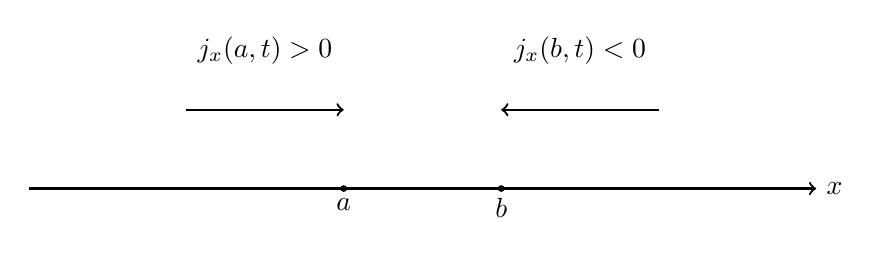
\begin{tikzpicture}
\draw[black,  thick, ->] (-3,0) -- (-1,0)  node[] at (2, 0.75) {$j_x(b,t)<0$};
\draw[black,  thick, ->] (3,0) -- (1,0)  node[] at (-2, 0.75) {$j_x(a,t)>0$};
\draw[black,  thick, ->] (-5,-1) -- (5,-1)  node[anchor=west]{$x$};
\filldraw[black] (1,-1) circle (1pt) node[anchor=north]{$b$};
\filldraw[black] (-1,-1) circle (1pt) node[anchor=north]{$a$};
\end{tikzpicture}
\caption{\textit{sannsynlighetsstrømmen inn og ut av et område $[a,b]$ bestemmer hvordan 
sannsynlighetstettheten endrer seg på intervallet. Hvis e.g. $j_x(b,t)$ er negativ 
flyter sannsynlighetstrømmen inn i intervallet og det blir mer sannsynlig at partikkelen finnes der.
Tilsvarende hvis $j_x(a,t)$ er positiv, da flyter sannsynlighetstrømmen inn i $[a,b]$.}}
\label{fig:j_x}
\end{figure}

\subsection{Heisenberg's Uskarphetsrelasjon}
Hvis vi ser for oss en bølge med en enkelt bølgelengde så kan vi lett måle bølgens bølgelengde 
men ikke hvor bølgen er; bølgen er over alt. 
På den andre siden kan vi se for oss en partikkel; den er er helt nøyaktig lokalisert i rommet,
men vi kan ikke bestemme bølgelengden til partikkelen. Siden vi vet at bevegelsesmengden til 
partikkelen er gitt ved  $p=\frac{h}{\lambda}$ har vi da at bevegelsesmengden ikke kan bestemmes 
entydig. \\

Vi har sett at planbølger på formen 
\begin{align}
	 \Psi(x,t) = Ce^{i(kx - \omega t)}
\end{align}
er løsninger til S.L., men vi ser fort at dette er problematisk siden vi har sagt at bare kvadrat 
integrerbare bølgefunksjoner er fysikalske. Vi ser at planbølger ikke er kvadrat integrerbar og
ikke kan normaliseres siden de ikke går mot 0 når $|x| \to \infty$ som vi ser i Fig.~\ref{fig:non_norm}. 
I tillegg kan vi ikke bestemme posisjonen til en planbølge siden den er overalt i rommet, 
og vi ønsker å kunne betrakte lokaliserte partikler.

Men vi vet at S.L. er lineær og hvis vi har to løsninger av S.L. så er lineær kombinasjon av de 
også en løsning. Vi kan overlagre bølger og skape noe som er mer lokalisert i rommet, som vi ser 
antydninger til i Fig.~\ref{fig:superposition}. Vi har at for 4 overlagrede bølger kan vi skape en 
ganske lokalisert puls, men som gjentas i det uendelige.
\begin{figure}[h!]
     \centering
     \begin{subfigure}[b]{0.8\textwidth}
       \centering
	\begin{tikzpicture}[width=\textwidth]
	  \begin{axis}%
	    [grid=both,
	     minor tick num=1,
	     xlabel=$x$,
	     ylabel=$y$,
	     grid style={line width=.01pt, draw=gray!10},
	     major grid style={line width=.2pt,draw=gray!50},
	     axis lines=middle,
	     restrict y to domain=-1:1.,
	     enlargelimits={abs=1.25}
	    ]
	    \addplot+[mark=none, 
		    domain=-4:4,
		    samples=150,
		    hatch distance=5pt,
		    hatch thickness=0.5pt,
		    draw=red!70,
		    pattern color=blue,
		    area legend] {cos(deg(pi*x))}  node[pos=1] (endofplot) {};
	    \node [above, color=red!70] at (endofplot) {$\cos(kx)$};
	    \addplot+[mark=none, 
		    domain=-4:4,
		    samples=150,
		    hatch distance=5pt,
		    hatch thickness=0.5pt,
		    draw=blue!70,
		    pattern color=blue,
		    area legend] {cos(deg(pi*x))^2}  node[pos=0] (endofplot_1) {};
	    \node [above, color=blue!70] at (endofplot_1) {$\cos^2(kx)$};
	  \end{axis}
	\end{tikzpicture}
         \caption{$y=\cos(kx)$ og $y' = \cos^2(kx)$}
         \label{fig:non_norm}
     \end{subfigure}
     \hspace{4cm}
     \begin{subfigure}[b]{0.3\textwidth}
         \centering
	\begin{tikzpicture}[width=\textwidth]
	  \begin{axis}%
	    [grid=both,
	     minor tick num=1,
	     xlabel=$x$,
	     ylabel=$y$,
	     grid style={line width=.01pt, draw=gray!10},
	     major grid style={line width=.2pt,draw=gray!50},
	     axis lines=middle,
	     restrict y to domain=-2:2.,
	     enlargelimits={abs=2.}
	    ]
	    \addplot+[mark=none, 
		    domain=-35:35,
		    samples=350,
		    hatch distance=5pt,
		    hatch thickness=0.5pt,
		    draw=red!70,
		    pattern color=blue,
		    area legend] {cos(deg((pi + .4)*x)) + cos(deg(pi*x))} ;
	    \node [below, color=red!70] at (20, -2) {$\cos(kx) + \cos(k'x)$};
	  \end{axis}
	\end{tikzpicture}
         \caption{$y=\cos(kx) + \cos(k'x)$}
         \label{fig:2super}
     \end{subfigure}
     \hspace{3cm}
     \begin{subfigure}[b]{0.3\textwidth}
         \centering
	\begin{tikzpicture}[width=\textwidth]
	\begin{axis}%
	[grid=both,
	minor tick num=1,
	xlabel=$x$,
	ylabel=$y$,
	grid style={line width=.01pt, draw=gray!10},
	major grid style={line width=.2pt,draw=gray!50},
	axis lines=middle,
	restrict y to domain=-4:4.,
	enlargelimits={abs=2.}
	]
	\addplot+[mark=none, 
	    domain=-35:35,
	    samples=350,
	    hatch distance=5pt,
	    hatch thickness=0.5pt,
	    draw=red!70,
	    pattern color=blue,
	    area legend] {cos(deg((pi + .2)*x)) + cos(deg(pi*x)) +
			  cos(deg((pi + .4)*x)) + cos(deg((pi + 0.6)*x))} ;
	\node [below, color=red!70] at (1, -4) {$\cos(kx) + \cos(k'x)  + \cos(k''x) + \cos(k'''x)$};
	\end{axis}
	\end{tikzpicture}
         \caption{$y=\cos(kx) + \cos(k'x) + \cos(k''x) + \cos(k'''x)$}
         \label{fig:4super}
     \end{subfigure}
        \caption{Ovelagring av cosinus bølger.}
        \label{fig:superposition}
\end{figure}
Hvis vi overlagrer uendelig mange bølge kan vi skape en puls som gjentas uendelig sjelden, dvs som er 
lokalisert rundt ett området i rommet. 
Siden vi trenger uendelig mange overlagrede bølger blir summen vår til et integral, og vi har 
\begin{align}
	 \Psi(x,t) = \int_{-\inty}^{\infty} A(k)e^{i(kx - \omega(k) t)} dk
\end{align}
hvor vi inkluderer alle mulige bølgelengder ved at vi integrerer over $k$. Dette er nå noe som kan være 
lokalisert, gitt at $A(k)$ er det. 

Vi skal nå se på en Gaussisk bølgepakke, hvor vi lar $A(k)$ ha formen til en Gauss-kurve, vi har da 
\begin{align}
	 A(k) = \frac{\sqrt{\sigma}}{\sqrt{2}\pi^{\frac{1}{4}} } e^{-(k-k_0)^2 \frac{\sigma^2}{2}}
\end{align}
hvor $\sigma$ er bredden til Gauss-kurven og $k_0$ bølgetallet som kurven er sentrert rundt. 
Vi har nå følgende bølgefunksjon
\begin{align}
	 \Psi(x, t) = \frac{\sqrt{\sigma}}{\sqrt{2}\pi^{\frac{1}{4}} } \int_{-\infty}^{\infty} 
	e^{-(k-k_0)^2 \frac{\sigma^2}{2}} e^{i(kx - \omega(k)t)} dk
\end{align}
Dette tilfredstiller åpenbart S.L. siden vi vet at den er lineær og vi har har en sum linearkombinasjon
av løsninger til S.L. (et integral, men som vi kan se på som en kontinuerlig sum).


\end{document}

